% Authors: Anwar Baroudi
% Emails: mabaroudi@berkeley.edu


\qns{Least Squares}

\meta{\\
Prereqs: Understanding of the mechanics and interpretations of (L2) norms
}
\ans{\\
Description: Describe and derive the least squares problem and solution, first geometrically, and then using calculus.
}
\begin{enumerate}



\begin{figure}[H]
	\begin{center}
		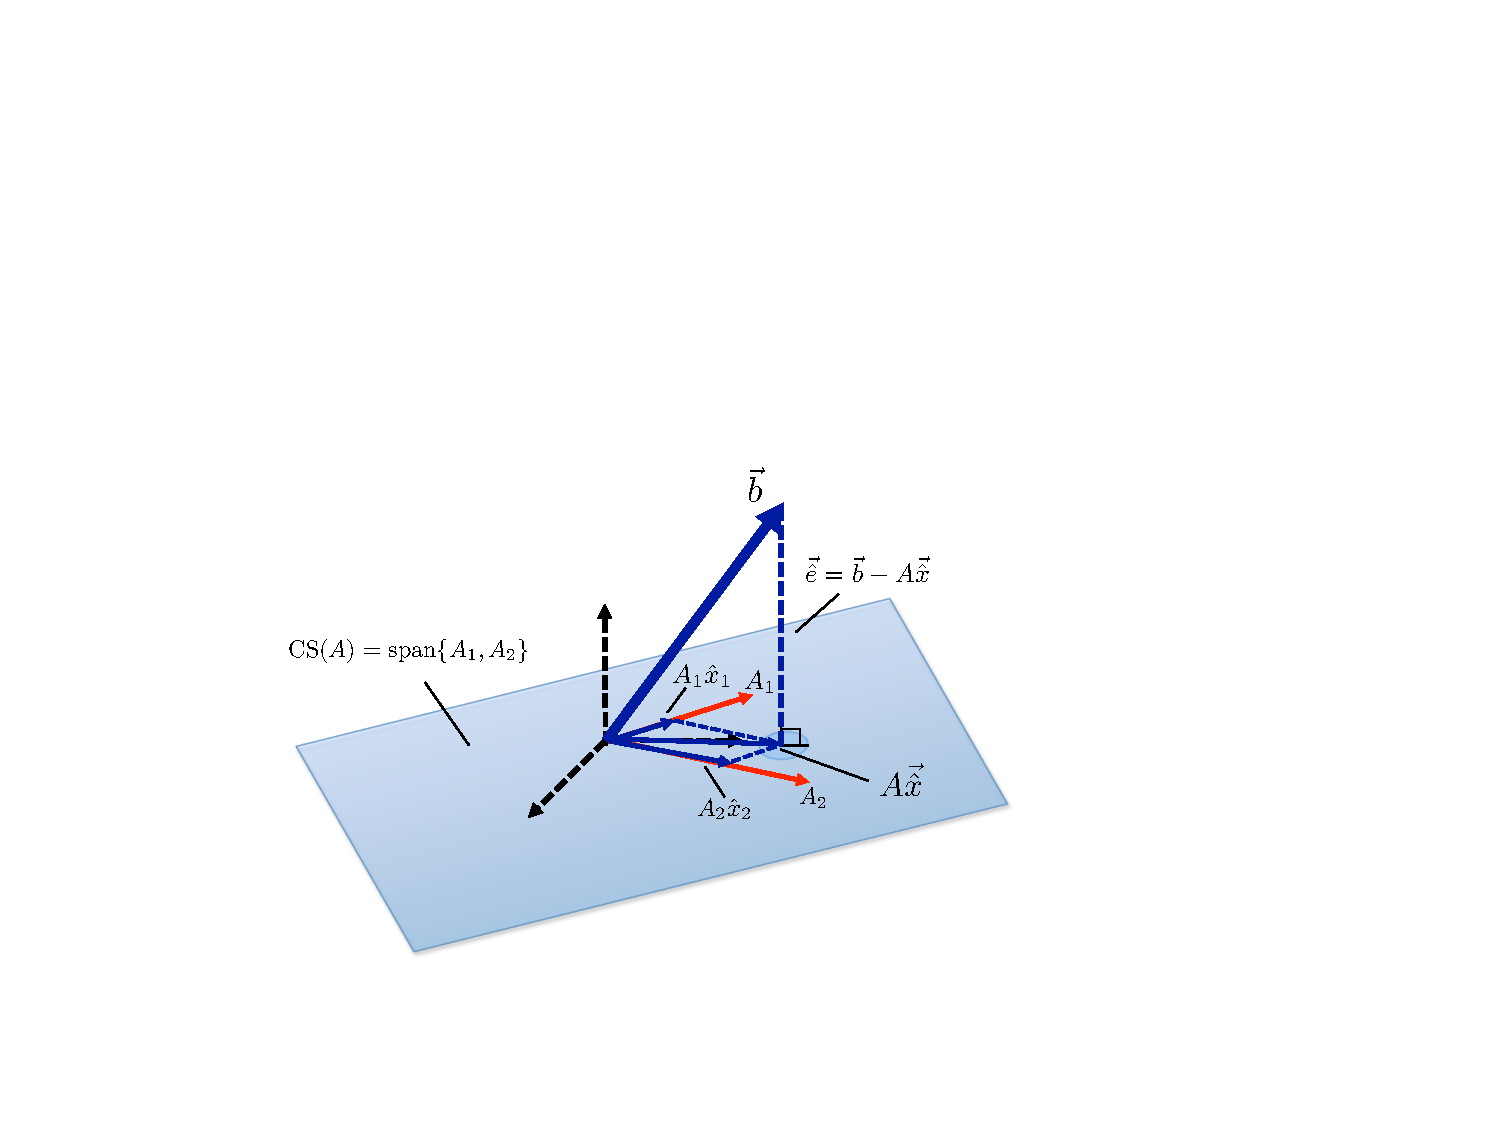
\includegraphics[]{figs/LS_gen_sol.pdf}
	\end{center}
\end{figure}
\qitem{}
Consider that you have some equations of the form $\mathbf{A}\vec{x} = \vec{b}$, however, that there is no solution $\vec{x}$ that solves the equations. What does this tell us about $\vec{b}$ with respect to $\mathbf{A}_1, \mathbf{A}_2$ (the columns of \mathbf{A})?

\ans{$\vec{b}$ is not in the column space of $\mathbf{A}$. If there was some $\vec{x}$ which solved the equation $\mathbf{A}\vec{x} = \vec{b}$, then we could write $\vec{b} = \mathbf{A}_1 x_1 + \mathbf{A}_2 x_2$, and $\vec{b}$ would have been in the column space of $\mathbf{A}$. However, since there is no such $\vec{x}$, $\vec{b}$ is not in the column space of \mathbf{A}.}

\qitem{
We know that there is no $\vec{x}$ that satisfies the equations exactly, but we still want to solve the equations to get a solution as close as possible.

Let's say you had 3 choices, $\vec{x}_i, \vec{x}_j, \vec{x}_k$ (these are not drawn on the image). Which one would you pick?
}

\meta{Be very careful. The word 'close' is used here, on purpose, since the kind of error has not yet been defined. When teaching this, make sure to use the word 'close' as intended.}

\ans{A good idea would be to multiply out $\mathbf{A}\vec{x}_i, \mathbf{A}\vec{x}_j, \mathbf{A}\vec{x}_k$, and see which one results in something closest to $\vec{b}$, and that's the one that we would pick.}

\qitem{Suppose that the real $\vec{b} = \begin{bmatrix} 2 \\ 1 \end{bmatrix}$, and you have two close $\vec{x}_1, \vec{x}_2$, which result in possible $\vec{b}_1 = \begin{bmatrix} 1.5 \\ 1.5 \end{bmatrix}$ and another $\vec{b}_1 = \begin{bmatrix} 1 \\ 1 \end{bmatrix}$. How do we know which one is \textit{closer}? What if we define \textit{closer} to mean the sum of the components of the difference of the vectors.}

\meta{This is pretty much walkthrough, although the reason it is written as a question is so that students can get a chance to come with up some reasons themselves.}

\ans{
There are many ways to define closeness. One way is to simply sum up the differences in individual entries. For instance, the sum of the entries in $\vec{b} - \vec{b}_1$ vs. the sum of the entries in $\vec{b} - \vec{b}_2$. The first sum equals 0, while the second one equals 1. Huh? Both of these vectors seemed like they were '1' unit away, but the first one results in a sum of 0. This is because of negative numbers. 

$\vec{b}_1$ is -0.5 away in the first element, and 0.5 away in the second. We should interpret this as being 1 away. In other words, we should take the absolute value of the differences of the individual elements. It turns out that this is, mathematically, annoying. 
}

\qitem{What is a different approach to solve the issue discussed above?}

\ans{
Another way to get rid of negative numbers is by simply squaring the element-wise difference. Define the 'closeness' by the 'sum of the squares of individual elements in the vectors'.
}
    
\qitem{Using this definition, how close is $\vec{b}_1$ to $\vec{b}$? How close is $\vec{b}_2$ to $\vec{b}$?}

\ans{
$\vec{b}_1$: $-0.5^2 + 0.5^2 = 0.5$ and $\vec{b}_2$: $1^2 + 0^2 = 1$. Using this definition, $\vec{b}_1$ is closer, and that's the one we should pick!
}

\qitem{
More generally, we actually don't have a choice of just two or three $\vec{x}$s to pick to get as close to $\vec{b}$ as possible. We have an infinite number of choices. How can we tell which one is the best? Look at the image given at the top of the question, and decide something about $\vec{\hat{x}}$ and $\vec{\hat{e}}$}.

\ans{
We want to pick an $\vec{\hat{x}}$ which results in the smallest norm-squared of $\vec{\hat{e}}$.

$\vec{\hat{e}}$ is exactly the 'difference' that we discussed earlier of the correct $\vec{b}$ and the closest vector that we can get to $\vec{b}$. The norm-squared of $\vec{\hat{e}}$ is precisely the sum of squares of the elements in the difference. We want to minimize $\vec{\hat{e}}$. 
}

\qitem{
Let's begin by recalling three facts. Recall that if we want to minimize some quantity squared, it is enough to minimize the quantity itself. Also, recall that given a point and a plane, the shortest line that one can possibly get starting at the point and ending at the plane, is a perpendicular line from the point to the plane. Finally, recall that the subspace which is orthogonal to the column space of some matrix $\mathbf{A}$ is the left-nullspace of $\mathbf{A}$. Using this information, come up with a method to minimize the norm-squared of $\vec{\hat{e}}$.}

\meta{The clause on minimizing some quantity squared only applies to positive values, but for the purposes of least squared, the values (lengths) are always positive anyway.}

\ans{
To minimize the norm-squared of $\vec{\hat{e}}$, we just want $\vec{\hat{e}}$ to be perpendicular to the column space of $\mathbf{A}$. This is the shortest-length (or smallest-norm) $\vec{\hat{e}}$ possible. Since finding the shortest-length vector is the same thing as minimizing the norm, which is equivalent to minimizing the norm-squared. 

To make this vector orthogonal to the column space of $\mathbf{A}$, it should be in the left-nullspace of $\mathbf{A}$, or $\mathbf{A}^T(\mathbf{A}\vec{\hat{x}} - \vec{\hat{x}}) = \vec{0}$. This says $\mathbf{A}^T\mathbf{A}\vec{\hat{x}} = \mathbf{A}^T\vec{\hat{b}}$.

The best $\vec{\hat{x}}$ we can find is $(\mathbf{A}^T\mathbf{A})^{-1}\mathbf{A}^T\vec{b}$.
}

    
\end{enumerate}